

\documentclass{article}
\usepackage[utf8]{inputenc}
\usepackage[danish]{babel}
\usepackage[T1]{fontenc}
\thispagestyle{empty}	
\usepackage{amsmath}	
\usepackage[paperwidth=14cm, paperheight=10cm,margin =0cm]{geometry}
\usepackage{tikz}
\usepackage{float}
\usepackage{pgfplots}
\usepackage{pgfplotstable}
\pgfplotsset{compat=newest}

\usetikzlibrary{shapes,shadows,arrows}
\newcommand{\dsplinewidth}{0.25mm}           % Line width for connections
\newcommand{\dspblocklinewidth}{0.3mm}       % Line width for blocks
\newcommand{\dspoperatordiameter}{4mm}       % Diameter for adder, multiplier, mixer
\newcommand{\dspoperatorlabelspacing}{2mm}   % Distance from symbol to label for adder, multiplier, mixer
\newcommand{\dspnoderadius}{1mm}             % Filled and empty node
\newcommand{\dspsquareblocksize}{8mm}        % Size for square blocks, e.g. for delay elements, decimator, expander
\newcommand{\dspfilterwidth}{14mm}           % Width of a filter block

	
\tikzstyle{dspsquare} = [shape=rectangle,draw=black,align=center,text depth=0.3em,text height=1em,inner sep=0pt,
	line cap=round,line join=round,line width=\dspblocklinewidth,minimum size=\dspsquareblocksize]
\tikzstyle{dspmultiplier} = [regular polygon, regular polygon sides=3,align=center,text depth=0.3em,
              text height=1em,inner sep=0mm,
              draw, fill=white, line width=\dspblocklinewidth,     
              shape border rotate=-90]
\tikzstyle{dspadder} = [circle,draw=black, line width=\dspblocklinewidth] 

\begin{document}


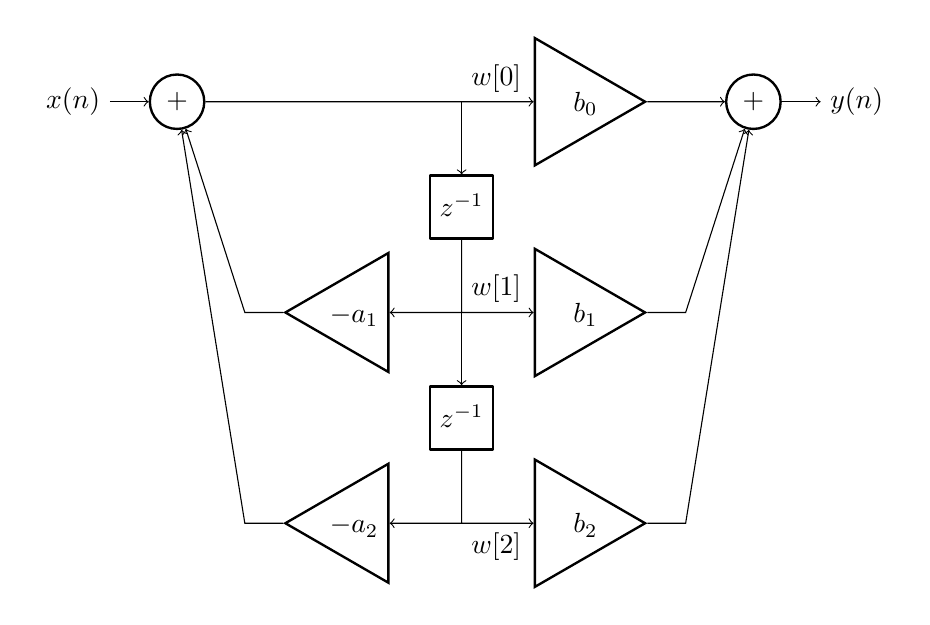
\begin{tikzpicture}[]

\matrix[column sep=5mm, row sep= 1mm] at (0,0)
{
    %------------------------------------------------------- 
 \node[]               (m00)   {$x(n)$};        &
 \node[dspadder]         (m01)     {$+$} ;     &
 \node[coordinate]             (m02)   {}; &
 \node[coordinate]               (m03)   {};&
\node[coordinate]               (m04)      {}; &
 \node[dspmultiplier]    (m05)       {$ \quad b_0 $};         &
 \node[coordinate]               (m06)       {}; &
 \node[dspadder]         (m07)       {$+$};    &
 \node[]               (m08)        {$y(n)$}; \\ 
%------------------------------------------------------- 
 \node[coordinate]               (m10)       {};        &
 \node[coordinate]               (m11)       {}; &
 \node[coordinate]                (m12)  {}; &
 \node[coordinate]   (m13) {}; &
 \node[dspsquare]         (m14)       {$z^{-1}$};     &
\node[coordinate]        (m15)       {};         &
 \node[coordinate]               (m16)        {}; \\ 
%------------------------------------------------------- 
\node[coordinate]         (m20)       { };            &
\node[coordinate]         (m21)        {}; &
\node[coordinate]         (m22)        {}; &
\node[dspmultiplier,shape border rotate=90]  (m23)    {$-a_1$}; &
\node[coordinate]         (m24)       {};     &
\node[dspmultiplier]     (m25)       {$\quad b_1$};           &
\node[coordinate]       (m26)       { };             \\   
%------------------------------------------------------- 
\node[coordinate]         (m30)       { };            &
\node[coordinate]         (m31)        {}; &
\node[coordinate]         (m32)        {}; &
\node[coordinate]  (m33)    {}; &
\node[dspsquare]         (m34)       {$z^{-1}$};     &
\node[coordinate]      (m35)       {};           &
\node[coordinate]       (m36)       { };             \\  
%------------------------------------------------------- 
\node[coordinate]         (m40)       { };            &
\node[coordinate]         (m41)        {}; &
\node[coordinate]         (m42)        {}; &
\node[dspmultiplier,shape border rotate=90]  (m43)    {$-a_2$}; &
\node[coordinate]        (m44)       {};     &
\node[dspmultiplier]     (m45)       {$\quad b_2$};           &
\node[coordinate]       (m46)       { };             \\    
};

% 1. column
\draw [->] (m00) -- (m01);
\draw [->] (m01) -- (m05);
\draw [->] (m04) node[anchor = south west]{$w[0]$} -- (m14);
\draw [->] (m05) -- (m07);
\draw [->] (m07) -- (m08);
% 2. column
\draw [->] (m14) -- (m24) -- (m25);
\draw [->] (m24) node[anchor =south west]{$w[1]$} -- (m23);
% 3. column
\draw [->] (m24) -- (m34);
\draw [->] (m25) -- (m26) -- (m07);
\draw [->] (m23) -- (m22) -- (m01);

% 4. column
\draw [->] (m34) -- (m44) -- (m45);
\draw [->] (m44)  node[anchor=north west]{$w[2]$} -- (m43);
\draw [->] (m43) -- (m42) -- (m01);
\draw [->] (m45) -- (m46) -- (m07);
\end{tikzpicture}

\end{document}